%% 
%% Copyright 2007, 2008, 2009 Elsevier Ltd
%% 
%% This file is part of the 'Elsarticle Bundle'.
%% ---------------------------------------------
%% 
%% It may be distributed under the conditions of the LaTeX Project Public
%% License, either version 1.2 of this license or (at your option) any
%% later version.  The latest version of this license is in
%%    http://www.latex-project.org/lppl.txt
%% and version 1.2 or later is part of all distributions of LaTeX
%% version 1999/12/01 or later.
%% 
%% The list of all files belonging to the 'Elsarticle Bundle' is
%% given in the file `manifest.txt'.
%% 
%% Template article for Elsevier's document class `elsarticle'
%% with harvard style bibliographic references
%% SP 2008/03/01

%\documentclass[preprint,12pt,authoryear]{elsarticle}  %default in the template
%\documentclass[preprint,10pt,authoryear]{elsarticle}

%% Use the option review to obtain double line spacing
%% \documentclass[authoryear,preprint,review,12pt]{elsarticle}

%% Use the options 1p,twocolumn; 3p; 3p,twocolumn; 5p; or 5p,twocolumn
%% for a journal layout:
%% \documentclass[final,1p,times,authoryear]{elsarticle}
%% \documentclass[final,1p,times,twocolumn,authoryear]{elsarticle}
 \documentclass[final,3p,times,authoryear]{elsarticle}
%% \documentclass[final,3p,times,twocolumn,authoryear]{elsarticle}
%% \documentclass[final,5p,times,authoryear]{elsarticle}
%% \documentclass[final,5p,times,twocolumn,authoryear]{elsarticle}

%% For including figures, graphicx.sty has been loaded in
%% elsarticle.cls. If you prefer to use the old commands
%% please give \usepackage{epsfig}

%% The amssymb package provides various useful mathematical symbols
\usepackage{amssymb}
%% The amsthm package provides extended theorem environments
\usepackage{amsthm}
\usepackage{amsmath}
\usepackage{color, colortbl}
\usepackage{amsmath}
\usepackage{siunitx}
%\usepackage{todonotes}
\usepackage{tabularx}
\usepackage[]{algorithm2e}
\usepackage{soul}
%\usepackage[colorinlistoftodos]{todonotes}

\usepackage{glossaries}

\usepackage{xargs}
\usepackage[pdftex,dvipsnames]{xcolor}
\usepackage[colorinlistoftodos,prependcaption,textsize=tiny]{todonotes}
\newcommandx{\unsure}[2][1=]{\todo[linecolor=red,backgroundcolor=red!25,bordercolor=red,#1]{#2}}
\newcommandx{\change}[2][1=]{\todo[linecolor=blue,backgroundcolor=blue!25,bordercolor=blue,#1]{#2}}
\newcommandx{\info}[2][1=]{\todo[linecolor=OliveGreen,backgroundcolor=OliveGreen!25,bordercolor=OliveGreen,#1]{#2}}
\newcommandx{\improvement}[2][1=]{\todo[linecolor=Plum,backgroundcolor=Plum!25,bordercolor=Plum,#1]{#2}}
\newcommandx{\thiswillnotshow}[2][1=]{\todo[disable,#1]{#2}}

\definecolor{light-gray}{gray}{0.9}

\usepackage{framed} % Framing content
\usepackage{multicol} % Multiple columns environment


\DeclareRobustCommand{\hlgreen}[1]{{\sethlcolor{green}\hl{#1}}}

\journal{TBD}
\makeglossaries


\begin{document}

%\runninghead{Nice et al.}

\title{Targeted urban heat mitigation strategies using urban morphology databases and micro-climate modelling to examine the urban heat profile}

\author[melb]{Kerry~A.~Nice\corref{cor1}}
\ead{kerry.nice@unimelb.edu.au}
\author[melb]{et al.}
%\author[melb]{Sachith Seneviratne}
%\author[melb]{Jasper S. Wijnands}
%\author[melb]{Jason Thompson}
%\author[melb,eng]{Mark Stevenson}
\cortext[cor1]{Principal corresponding author}
\address[melb]{Transport, Health, and Urban Design Hub, Faculty of Architecture, Building, and Planning, University of Melbourne, Australia.}
%\address[eng]{Melbourne School of Engineering; and Melbourne School of Population and Global Health, University of Melbourne, Australia.}







\begin{abstract}
TODO update

Strategies for urban heat mitigation often make broad and non-specific recommendations (i.e. plant more trees) without accounting for local context. As a result, resources might be allocated to areas of lesser need over those where more urgent interventions are needed. Also, these interventions might return less than optimal results if local conditions are not considered. This project aims to assist with these interventions by providing a method to examine the urban heat profile of a city through an automated systematic approach. Using urban morphology information from databases such as WUDAPT and Geoscape, areas of cities are clustered using a self organising map into distinct micro climate zones (MCZs) and modelled at a micro-scale using localised features and properties. This bottom up modelling approach, using the VTUF-3D, UMEP, and TARGET models, allows these areas to be assessed in detail for their human thermal comfort performance and provide a city-wide heat map of thermal comfort. The MCZ approach allows greater efficiency in modelling at a micro-scale, as fewer representative locations need to be modelled. It also allows mitigation scenarios to be tested and targeted for each cluster type. Case studies performed using this method for the Australian capital cities, Brisbane, Melbourne, Sydney, Perth, and Adelaide are presented.
\end{abstract}

\begin{keyword}
micro-climate\sep 
urban morphology\sep
urban heat
\end{keyword}



\maketitle





\section{Introduction}
TODO
   

Local climate zones based on clustering areas

Micro climate zones, based on clustering based on outcomes.

\section{Methods}\label{sec:methods}

\subsection{Scenario generation}\label{sec:methodsgen}
This study starts with Geoscape \citep{Geoscape2020} data from Public Sector Mapping Agency (PSMA) Australia. Geoscape provides 2 meter resolution land cover (road, building, grass, bare earth, etc) as well as building and tree footprints and heights (figure \ref{fig:geoscape}). Using this dataset for Melbourne, representative ranges were found for surface covers and tree and building heights and footprints. From these, 9814 model domains were created with all iterations (by 5\% increments) of fractions of trees, grass, buildings and streets, as well as average building heights (from 0 to 49 meters) and vegetation heights (from 0 to 20 meters in 0.5m increments) (figure \ref{fig:scenarios}). Domains were created of 100$\times$100m with 5m resolution grids.



\begin{figure*}
\centering
\includegraphics[page=2,trim={70 345 60 360},clip,scale=0.65]{Figures/Figures.pdf}
\caption{\bf 2m surface cover (bare earth, roads, grass, trees, water, and buildings), building footprints and heights, and tree cover locations and heights from Geoscape for Melbourne.}
 \label{fig:geoscape}
\end{figure*} 

\begin{figure*}
\centering
\includegraphics[page=3,trim={55 240 60 240},clip,scale=0.65]{../Presentation/PresentationImages.pdf}
\caption{\bf Melbourne, parameter ranges.}
\end{figure*} 

\begin{figure*}
\centering
\includegraphics[page=1,trim={70 380 60 390},clip,scale=0.65]{Figures/Figures.pdf}
\caption{\bf Melbourne, creation of VTUF-3D scenarios for 9814 variations of parameters.}
 \label{fig:scenarios}
\end{figure*} 






\subsection{VTUF-3D}\label{sec:methodsvtuf}
VTUF-3D \citep{Nice2018a} was used as the micro-climate modelling tool for this study. VTUF-3D is a urban micro-climate surface energy balance model that incorporates vegetation physiological processes and shading effects. The model provides output of canyon averaged air temperature ($T_{can}$) as well as 5m resolution values for each surface of surface temperature ($T_{surf}$), mean radiant temperature ($T_{mrt}$), and universal thermal climate index ($UTCI$) (figure \ref{fig:vtufresults}). Each model run was forced by the observations of Preston in Melbourne from \cite{Coutts2007} over the days February 9-14, 2004. 

An analysis time was used of  4 pm of February 12th. The current forcing conditions at that point were downward shortwave (\gls{kdown}) of 501.7$Wm^{-2}$, downward longwave (\gls{ldown}) of 365.1$Wm^{-2}$, air temperature of 25.9\SI{}{\degreeCelsius}, vapour pressure of 1.16 $mb$, wind at 173$^{\circ}$ of 5.4 $ms^{-1}$ and air pressure of 995.5$mb$. Energy balance parameters for net radiation (\gls{qstar}), sensible fluxes (\gls{qh}), ground flux (\gls{qg}), and latent heat (\gls{qe}) were also extracted, as well as shortwave and longwave up (\gls{kup} and \gls{lup}) (all in $Wm^{-2}$) and canyon wind speed ($U_{road}$) (in $ms^{-1}$).

\begin{figure*}
\centering
\includegraphics[page=2,trim={75 240 60 240},clip,scale=0.55]{../Presentation/PresentationImages.pdf}
\caption{\bf Melbourne, VTUF-3D results.}
 \label{fig:vtufresults}
\end{figure*} 

\subsection{Parameter analysis}\label{sec:methodsparam}
% analysis
% ProcessMCZResults.java
% -  temperature distributions at 0m created for each completed run
%  All surfaces at 0m for each timestep, temperatures and counts of for Tsfc, Tmrt, and UTCI.
%  Ta is single value (canyon averaged) for each domain
% - All runs are combined into single data file for each timestep
%     contains temperatures and energy fluxes

Domain mean values at ground surface level were calculated from the results from each scenario for for the parameters of $T_{can}$, $T_{surf}$, $T_{mrt}$, and $UTCI$ (all in $^{\circ}$C). 

Results from the 9814 completed model runs were extracted for each hourly timestep including the values for \gls{tsfc}, \gls{tmrt}, and \gls{utci} at ground level. VTUF-3D generates a single canyon averaged air temperature (\gls{tcan}). Additionally, domain averaged energy flux values were extracted, including latent fluxes (\gls{qe}), sensible fluxes (\gls{qh}), net radiation (\gls{qstar}), ground fluxes (\gls{qg}), shortwave up (\gls{kup}), shortwave down (\gls{kdown}), longwave up (\gls{lup}), and longwave down (\gls{ldown}). Hourly results were combined and indexed by their unique parameter ranges.

\subsection{Feature importance}\label{sec:methodsfeat}
%
% Feature importance
% /media/kerryn/87d9469d-56aa-4a1f-a62d-5f03d7599bbf/Data/VTUF-3D/Output/FeatureImportance/rf_all_runszslice.py
% feature_imporantance from RandomForestClassifier was used from scikit-learn \citep{scikit-learn}
% determine feature importance for paramaters of percentages of grass, trees, buildings, and roads, as well as average vegetation and building heights for Tair, Tsfc, Tmrt, and UTCI.

A feature importance analysis was performed using the Random Forest Classifier from  scikit-learn \citep{scikit-learn}. Ranks of feature importance were determined for each temperature type (\gls{tcan}, \gls{tsfc}, \gls{tmrt}, and \gls{utci}) for the four surface fraction parameters (grass, trees, buildings, and roads) as well as average vegetation and building heights.


\subsection{Temperature trends due to surface fractions and average heights}\label{sec:methodstempvspercent}

% 
% box_montage_reverse_zslice.sh
% plot_box_unclustered_tempRangeszSlice.py -> plot_box_reverse_6zSlice.py
% matplotlib used to plot hourly results for all scenarios for 4 temperature types
%  box plots made of temperatures vs percentages (by 10 %) of surfaces (tree, grass, building, road) and ave heights (by 0.4m) of vegetation and buildings
%  background colors of each plot were tinted by levels of feature importance.

To determine the trends of the four temperature types (\gls{tcan}, \gls{tsfc}, \gls{tmrt}, and \gls{utci}), Matplotlib \citep{Hunter2007} was used to generate box plots of modelled temperature results vs surface types (tree, grass, building, road) in 10\% ranges as well as average building and vegetation heights (in 0.4m ranges). The backgrounds of each plot were tinted in green according to the parameter's calculated level of feature importance.



\subsection{Distributions of temperatures across a diurnal cycle}\label{sec:methodsdist}
%
% ridge plots, ggridge_plots.R
%   sample scenarios were selected (that represented some of the most common urban arrangments)
%   hourly distributions on Feb 12 of Tsfc, Tmrt, and UTCI (Ta is only canyon averages) using R ggplot ggridges
% 

A number of scenarios were selected that represented frequent urban morphologies found in Melbourne and hourly distributions over a diurnal cycle (of February 12th) using ggridges \citep{ggridges}. Temperatures plotted were \gls{tsfc}, \gls{tmrt}, and \gls{utci}. \gls{tcan} is a single canyon average so does not have a distribution.


\subsection{City scale heat maps from micro-climate modelled results}\label{sec:methodsheatmaps}
% city heat maps
%  the vtuf scenarios used forcing (and range of urban morphologies) from Melbourne (Preston) Coutts 2007
%  completed model results were matched back to locations across Melbourne by matching the modelled parameters 
%   of surface fractions and heights to the actual parameters of those locations.
%  resulting heat maps of Ta, Tsfc, Tmrt, and UTCI were visualised in QGIS.
%  Tsfc results were compared to CSIRO LST maps generated by \citep{Devereux2017} and visialised in QGIS.
%  In addition, model results were matched to locations in Sydney, Perth, Brisbane, and Adelaide to generate heatmaps
%
%  

City-wide heat maps of \gls{tcan}, \gls{tsfc}, \gls{tmrt}, and \gls{utci} were generated from the 9814 modelled scenario results. Each model run was forced by the observations of Preston in Melbourne from \cite{Coutts2007} over the days February 9-14, 2004. The actual urban morphology parameters calculated from the Geoscape data were matched to the modelled scenario with the closest matching parameters of surface fractions and average heights for each 100$\times$100m location in Melbourne and visualized in QGIS \citep{QGIS2009}. Locations with greater than 10\% surface fraction of water were removed from the results as VTUF-3D does not currently model water bodies.

These resulting heatmaps show a city-wide assessment of thermal performance due to urban form but is independent of local weather conditions (i.e. ocean breezes vs. calm inland conditions). In addition, the same modelled results were matched to locations across Sydney, Perth, Brisbane, and Adelaide to generate city-wide urban form heatmaps for each of these cities.  \gls{tsfc} heatmap results were compared to the land surface temperature maps of \cite{Devereux2017}, which were generated from multiple aggregated Landsat 8 land surface temperature imagery over 2015-2016. Results were visialised in QGIS.

\section{Results}\label{sec:results}




\begin{figure*}
\centering
\includegraphics[page=1,trim={60 300 50 300},clip,scale=1.0]{Figures/Figures2.pdf}
\caption{\bf Surface fractions percentages and average heights vs. temperatures (\gls{tcan}, \gls{tsfc}, \gls{tmrt}, and \gls{utci}) for February 12, 2004, 12am. Feature importance for each temperature type is indicated by the green background tinting.}
 \label{fig:box0}
\end{figure*} 

\begin{figure*}
\centering
\includegraphics[page=2,trim={60 300 50 300},clip,scale=1.0]{Figures/Figures2.pdf}
\caption{\bf Surface fractions percentages and average heights vs. temperatures (\gls{tcan}, \gls{tsfc}, \gls{tmrt}, and \gls{utci}) for February 12, 2004, 5am. Feature importance for each temperature type is indicated by the green background tinting.}
 \label{fig:box5}
\end{figure*} 

\begin{figure*}
\centering
\includegraphics[page=3,trim={60 300 50 300},clip,scale=1.0]{Figures/Figures2.pdf}
\caption{\bf Surface fractions percentages and average heights vs. temperatures (\gls{tcan}, \gls{tsfc}, \gls{tmrt}, and \gls{utci}) for February 12, 2004, 2pm. Feature importance for each temperature type is indicated by the green background tinting.}
 \label{fig:box14}
\end{figure*} 


\begin{figure*}
\centering
\includegraphics[page=4,trim={60 180 50 180},clip,scale=0.8]{Figures/Figures2.pdf}
\caption{\bf Surface fractions percentages and average heights vs. temperatures (\gls{tcan} and \gls{tsfc}) for February 12, 2004, 12am. Feature importance for each temperature type is indicated by the green background tinting.}
 \label{fig:box0a}
\end{figure*} 

\begin{figure*}
\centering
\includegraphics[page=5,trim={60 180 50 180},clip,scale=0.8]{Figures/Figures2.pdf}
\caption{\bf Surface fractions percentages and average heights vs. temperatures (\gls{tcan} and \gls{tsfc}) for February 12, 2004, 5am. Feature importance for each temperature type is indicated by the green background tinting.}
 \label{fig:box5a}
\end{figure*} 

\begin{figure*}
\centering
\includegraphics[page=6,trim={60 180 50 180},clip,scale=0.8]{Figures/Figures2.pdf}
\caption{\bf Surface fractions percentages and average heights vs. temperatures (\gls{tcan} and \gls{tsfc}) for February 12, 2004, 2pm. Feature importance for each temperature type is indicated by the green background tinting.}
 \label{fig:box14a}
\end{figure*} 



\begin{figure*}
\centering
\includegraphics[page=7,trim={60 250 63 266},clip,scale=0.8]{Figures/Figures2.pdf}
\caption{\bf Distribution of \gls{tsfc} across February 12, 2004 for scenario 50\% grass, 49.99\% trees, 0.01\% road, 0\% building, average vegetation height of 4m, and average building height of 0m.}
 \label{fig:dist}
\end{figure*}


\begin{figure*}
\centering
\includegraphics[page=8,trim={60 250 63 266},clip,scale=0.8]{Figures/Figures2.pdf}
\caption{\bf Distribution of \gls{tsfc} across February 12, 2004 for scenario 19\% grass, 10\% trees, 30\% road, 40\% building, average vegetation height of 2m, and average building height of 6m.}
 \label{fig:dist}
\end{figure*}



\begin{figure*}
\centering
\includegraphics[page=9,trim={60 250 63 266},clip,scale=0.8]{Figures/Figures2.pdf}
\caption{\bf Distribution of \gls{tsfc} across February 12, 2004 for scenario 29\% grass, 70\% trees, 1\% road, 0\% building, average vegetation height of 0.5m, and average building height of 0m.}
 \label{fig:dist}
\end{figure*}

\begin{figure*}
\centering
\includegraphics[page=10,trim={60 250 63 266},clip,scale=0.8]{Figures/Figures2.pdf}
\caption{\bf Distribution of \gls{tsfc} across February 12, 2004 for scenario 19\% grass, 10\% trees, 20\% road, 50\% building, average vegetation height of 1m, and average building height of 30m.}
 \label{fig:dist}
\end{figure*}


\begin{figure*}
\centering
\includegraphics[page=11,trim={60 250 63 266},clip,scale=0.8]{Figures/Figures2.pdf}
\caption{\bf Distribution of \gls{tsfc} across February 12, 2004 for scenario 89\% grass, 0\% trees, 8\% road, 3\% building, average vegetation height of 0m, and average building height of 5m.}
 \label{fig:dist}
\end{figure*}


\begin{figure*}
\centering
\includegraphics[page=12,trim={60 250 63 266},clip,scale=0.8]{Figures/Figures2.pdf}
\caption{\bf Distribution of \gls{tsfc} across February 12, 2004 for scenario 40\% grass, 10\% trees, 20\% road, 30\% building, average vegetation height of 2m, and average building height of 14m.}
 \label{fig:dist}
\end{figure*}

\begin{figure*}
\centering
\includegraphics[page=13,trim={60 250 63 266},clip,scale=0.8]{Figures/Figures2.pdf}
\caption{\bf Distribution of \gls{tsfc} across February 12, 2004 for scenario 19\% grass, 20\% trees, 21\% road, 40\% building, average vegetation height of 1m, and average building height of 9m.}
 \label{fig:dist}
\end{figure*}


\begin{figure*}
\centering
\includegraphics[page=14,trim={155 270 147 328},clip,scale=1.0]{Figures/Figures2.pdf}
\caption{\bf Air temperature heatmap on February 12, 2004 at 2pm generated by matching the closest matching parameters of surface fractions and average heights for each 100$\times$100m location in Melbourne from 9814 modelled scenario results.  }
 \label{fig:dist}
\end{figure*}

\begin{figure*}
\centering
\includegraphics[page=15,trim={155 270 141 328},clip,scale=1.0]{Figures/Figures2.pdf}
\caption{\bf Surface temperature heatmap on February 12, 2004 at 2pm generated by matching the closest matching parameters of surface fractions and average heights for each 100$\times$100m location in Melbourne from 9814 modelled scenario results.  }
 \label{fig:dist}
\end{figure*}

\begin{figure*}
\centering
\includegraphics[page=16,trim={155 290 124 329},clip,scale=1.0]{Figures/Figures2.pdf}
\caption{\bf Differences in surface temperature heatmap on February 12, 2004 at 2pm generated by matching the closest matching parameters of surface fractions and average heights for each 100$\times$100m location in Melbourne from 9814 modelled scenario results from land surface temperature maps of \cite{Devereux2017}.  }
 \label{fig:dist}
\end{figure*}


\begin{figure*}
\centering
\includegraphics[page=17,trim={155 255 141 328},clip,scale=1.0]{Figures/Figures2.pdf}
\caption{\bf Mean radiant temperature heatmap on February 12, 2004 at 2pm generated by matching the closest matching parameters of surface fractions and average heights for each 100$\times$100m location in Melbourne from 9814 modelled scenario results.  }
 \label{fig:dist}
\end{figure*}



\begin{figure*}
\centering
\includegraphics[page=18,trim={155 255 147 328},clip,scale=1.0]{Figures/Figures2.pdf}
\caption{\bf \gls{utci} temperature heatmap on February 12, 2004 at 2pm generated by matching the closest matching parameters of surface fractions and average heights for each 100$\times$100m location in Melbourne from 9814 modelled scenario results.  }
 \label{fig:dist}
\end{figure*}




\begin{figure*}
\centering
\includegraphics[page=19,trim={200 300 175 350},clip,scale=1.5]{Figures/Figures2.pdf}
\caption{\bf Air temperature heatmap on February 12, 2004 at 2pm generated by matching the closest matching parameters of surface fractions and average heights for each 100$\times$100m location in Sydney from 9814 modelled scenario results.  }
 \label{fig:dist}
\end{figure*}

\begin{figure*}
\centering
\includegraphics[page=20,trim={200 300 170 350},clip,scale=1.5]{Figures/Figures2.pdf}
\caption{\bf Surface temperature heatmap on February 12, 2004 at 2pm generated by matching the closest matching parameters of surface fractions and average heights for each 100$\times$100m location in Sydney from 9814 modelled scenario results.  }
 \label{fig:dist}
\end{figure*}

\begin{figure*}
\centering
\includegraphics[page=21,trim={200 290 170 280},clip,scale=1.5]{Figures/Figures2.pdf}
\caption{\bf Differences in surface temperature heatmap on February 12, 2004 at 2pm generated by matching the closest matching parameters of surface fractions and average heights for each 100$\times$100m location in Sydney from 9814 modelled scenario results from land surface temperature maps of \cite{Devereux2017}. TODO, yes I know degrees is misspelled in the image, will fix later. }
 \label{fig:dist}
\end{figure*}


\begin{figure*}
\centering
\includegraphics[page=22,trim={200 300 170 350},clip,scale=1.5]{Figures/Figures2.pdf}
\caption{\bf Mean radiant temperature heatmap on February 12, 2004 at 2pm generated by matching the closest matching parameters of surface fractions and average heights for each 100$\times$100m location in Sydney from 9814 modelled scenario results.  }
 \label{fig:dist}
\end{figure*}

\begin{figure*}
\centering
\includegraphics[page=23,trim={200 300 170 350},clip,scale=1.5]{Figures/Figures2.pdf}
\caption{\bf \gls{utci} heatmap on February 12, 2004 at 2pm generated by matching the closest matching parameters of surface fractions and average heights for each 100$\times$100m location in Sydney from 9814 modelled scenario results.  }
 \label{fig:dist}
\end{figure*}

\begin{figure*}
\centering
\includegraphics[page=24,trim={200 300 180 350},clip,scale=1.5]{Figures/Figures2.pdf}
\caption{\bf Air temperature heatmap on February 12, 2004 at 2pm generated by matching the closest matching parameters of surface fractions and average heights for each 100$\times$100m location in Perth from 9814 modelled scenario results.  }
 \label{fig:dist}
\end{figure*}

\begin{figure*}
\centering
\includegraphics[page=25,trim={200 300 180 350},clip,scale=1.5]{Figures/Figures2.pdf}
\caption{\bf Surface temperature heatmap on February 12, 2004 at 2pm generated by matching the closest matching parameters of surface fractions and average heights for each 100$\times$100m location in Perth from 9814 modelled scenario results.  }
 \label{fig:dist}
\end{figure*}

\printglossaries

\section*{References}\label{sec:ref}

  \bibliographystyle{elsarticle-harv} 
 % \bibliography{bib}
   \bibliography{BlockTypologies-EBP}




% % % %\nomenclature{$\alpha$}{shortwave albedo }
%\nomenclature{$\alpha_{sfc}$}{surface albedo (=0.15)} 
%\nomenclature{$\alpha_{g}$}{globe albedo (=0.05)} 
%\nomenclature{$\alpha _{veg}$}{shortwave albedo of vegetation}
%% % % %\nomenclature{$\epsilon$}{longwave emissivity}
%\nomenclature{$\epsilon _{veg}$}{longwave emissivity of vegetation}
%\nomenclature{$\epsilon_{a}$}{longwave emissivity of the atmosphere} 
%\nomenclature{$\epsilon_{g}$}{globe emissivity (=0.95)}  
%\nomenclature{$\sigma$}{Stefan-Boltzmann constant (=5.67 $\times$ 10$^{-8}$W m$^{-2}$K$^{-4}$)} 
%\nomenclature{$\theta$}{solar zenith angle} 
%\nomenclature{$A$}{surface area of a sphere of diameter D, of value 0.15m, (=$\pi 0.15^{2}$m$^{2}$)} 
%\nomenclature{$d$}{index of agreement (0 \textless= d \textless= 1)} 
%\nomenclature{$f_{dir}$}{fraction of the total horizontal solar irradiance, $S$, due to the direct beam of the sun}
%\nomenclature{$h$}{convective heat transfer coefficient (W m$^{-2}$K$^{-1}$)} 
%\nomenclature{$h_{i}$}{heat transfer coefficient (W m$^{-2}$K$^{-1}$)} 
%\nomenclature{$k$}{thermal conductivity of the fluid (i.e. air) (W m$^{-1}$ K$^{-1}$)} 
%\nomenclature{$K\downarrow_{dif}$}{domain-level incoming diffuse shortwave (W m$^{-2}$)}
%\nomenclature{$K\downarrow_{dir}$}{domain-level incoming direct shortwave (W m$^{-2}$)}
%\nomenclature{$K\downarrow$}{downward shortwave radiative flux density (W m$^{-2}$)} 
%\nomenclature{$L \downarrow_{i,sky}$}{initial incident sky-derived longwave (W m$^{-2}$)} 
%\nomenclature{$L\downarrow$}{downward longwave radiative flux density (W m$^{-2}$)}
%\nomenclature{$RMSE$}{root mean square error} 
%\nomenclature{$S$}{horizontal solar irradiance (W m$^{-2}$)} 
%\nomenclature{$T_{sfc,veg}$}{vegetation surface temperature (K)} 
%\nomenclature{$T_{sfc}$}{surface temperature (K)} 
%\nomenclature{$T_{g}$}{globe temperature (K)} 
%\nomenclature{$T_{a}$}{dry bulb air temperature (K)} 
%% % % %\nomenclature{$T_{s,1}$}{soil surface temperature (K)}
%% % % %\nomenclature{$T_{conv}$}{converging canyon temperature (K)} 
%\nomenclature{$Q^{*}_{veg}$}{calculation of vegetation net radiation flux density (W m$^{-2}$)}
%\nomenclature{$Q^{*}$}{net radiation flux density (W m$^{-2}$)} 
%\nomenclature{$Q_{E}$}{latent heat flux (W m$^{-2}$)}
%\nomenclature{$Q_{E,veg}$}{calculation of vegetation latent heat flux (W m$^{-2}$)} 
%\nomenclature{$Q_{F}$}{anthropogenic heat (W m$^{-2}$)}
%\nomenclature{$Q_{G}$}{ground heat storage (W m$^{-2}$)}
%\nomenclature{$Q_{G,veg}$}{calculation of vegetation ground heat storage (W m$^{-2}$)} 
%\nomenclature{$Q_{H}$}{sensible heat flux (W m$^{-2}$)} 
%\nomenclature{$Q_{H,veg}$}{calculation of vegetation sensible heat flux (W m$^{-2}$)} 
%\nomenclature{$ws_{cm}$}{wind speed (cm s$^{-1}$)} 
\newglossaryentry{utci}{name=$UTCI$,description={universal thermal climate index (\SI{}{\degreeCelsius})}}
\newglossaryentry{tsfc}{name=$T_{sfc}$,description={surface temperature (\SI{}{\degreeCelsius})}} 
\newglossaryentry{tcan}{name=$T_{can}$,description={canyon averaged air temperature (\SI{}{\degreeCelsius})}} 
\newglossaryentry{ta}{name=$T_{a}$,description={Air temperature (\SI{}{\degreeCelsius})}} 
\newglossaryentry{tmrt}{name=$T_{mrt}$,description={mean radiant temperature (\SI{}{\degreeCelsius})}} 

\newglossaryentry{qstar}{name=$Q^{*}$,description={net radiation flux density (W m$^{-2}$)}} 
\newglossaryentry{qe}{name=$Q_{E}$,description={latent heat flux (W m$^{-2}$)}} 
\newglossaryentry{qh}{name=$Q_{H}$,description={sensible heat flux (W m$^{-2}$)}} 
\newglossaryentry{qg}{name=$Q_{G}$,description={ground heat flux (W m$^{-2}$)}} 

\newglossaryentry{lup}{name=$L\downarrow$,description={upward longwave radiative flux density (W m$^{-2}$)}} 
\newglossaryentry{ldown}{name=$L\uparrow$,description={downward longwave radiative flux density (W m$^{-2}$)}} 
\newglossaryentry{kup}{name=$K\downarrow$,description={upward shortwave radiative flux density (W m$^{-2}$)}} 
\newglossaryentry{kdown}{name=$K\uparrow$,description={downward shortwave radiative flux density (W m$^{-2}$)}} 


\end{document}
